\documentclass{standalone}
\usepackage{tikz}
\usepackage{ctex,siunitx}
\setCJKmainfont{Noto Serif CJK SC}
\usepackage{tkz-euclide}
\usepackage{amsmath}
\usetikzlibrary{patterns, calc,3d}
\usetikzlibrary {decorations.pathmorphing,decorations.pathreplacing,decorations.shapes}
\begin{document}
\small
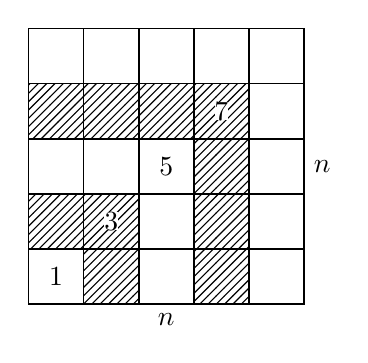
\begin{tikzpicture}[>=latex,scale=0.7]
  \fill[even odd rule,pattern=north east lines](0,0)rectangle(4,4)(0,0)rectangle(3,3)(0,0)rectangle(2,2)(0,0)rectangle(1,1);
  \foreach \x[count =\i] in {1,3,5,7}
  {
    \draw[semithick](\i,0)--(\i,5);
    \draw[semithick](0,\i)--(5,\i);
    \node at (\i-0.5,\i-0.5)[fill=white,inner sep=0pt]{\x};
  }
  \draw[semithick](0,0)rectangle(5,5);
  \node at (2.5,0)[below]{$n$};
  \node at (5,2.5)[right]{$n$};
\end{tikzpicture}
\end{document}